\documentclass{beamer}% тип документа
% далее идёт преамбула
\usepackage{blindtext}
\usepackage{hypcap}
\usepackage[T2A,T1]{fontenc}
\usepackage[utf8]{inputenc}
\usepackage[russian]{babel}
\usepackage{graphicx}
\usepackage{datetime}
\usepackage{multicol}




\begin{document}% начало презентации

\title{Разработка стохастической модели роста филамента в структуре оксидной пленки}
\author{Соловьёв Максим Андреевич}
\date{\today}
\institute{Кафедра физики твердого тела,
Физический факультет,\\
Московский государственный университет имени М.В.Ломоносовва.\\
Научный руководитель: кандидат физико-математических наук\\
    Бажанов Дмитрий Игоревич}



\begin{frame}% первый слайд
\begin{figure}
    \centering
    
\includegraphics[width=60px]{img/ff-sign.png}
\end{figure}
\maketitle
\end{frame}

\begin{frame}{Мемристор}
\begin{multicols}{2}
Мемристор - это пассивный элемент в микроэлектронике, способный изменять свое сопротивление в зависимости от протекающего через него заряда. 

\columnbreak
    \begin{figure}
        \centering
        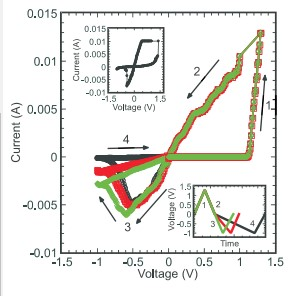
\includegraphics[width=160px]{img/vac_memrister.jpg}
        \caption{ВАХ мемристора%
    \footnote{%
    Journal of Vacuum Science and Technology B 29, 01AD03 (2011); doi: 10.1116/1.3521503
    }%
    }
    \end{figure}
\end {multicols}
\end{frame}

\begin{frame}{Мотивация}
\begin{multicols}{2}
Мемристор может быть использован как синапс в нейроморфных сетях, что является потенциально значимым применением элемента.

\columnbreak
    
    \begin{figure}
        \centering
        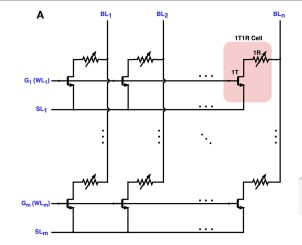
\includegraphics[width=160px]{img/sinaps-memristor-scheme.jpg}
        \caption{Принципиальная схема использования мемристора как синопса в нейроморфной сети%
        \footnote{%
        Guo* Y, Wu H, Gao B and Qian H(2019) Unsupervised Learning on Resistive Memory Array Based Spiking Neural Networks. Front. Neurosci. 13:812. doi: 10.3389/fnins.2019.00812
        }%
    }
    \end{figure}
\end{multicols}

\end{frame}


%Цель работы - что собираюсь делать и как моделировать
\begin{frame}{Цель работы}

Создание симулятора, позволяющего моделировать мемристор
и протекающие в нем процессы.
\begin{figure}
    \centering
    \includegraphics[width=300px]{schemes/model/model.pdf}
    \caption{
        Принципиальная схема симулятора
}
\end{figure}






\end{frame}

\begin{frame} {Реакции}

\begin{tabular}{p{3.3cm} | p{3.3cm}| p{3.3cm}}
    \textbf{Ионные реакции}
    \begin{itemize}
        \item Дрифт ионов в межузельные положения и обратно
        \item Образование пар ион-вакансия и рекомбинация
        
    \end{itemize} &
    \textbf{Электронный транспорт и динамика}
    \begin{itemize}
        \item Эмиссия шотки
        \item Эмиссия Пуля-Френкеля
        \item Туннелирование между ловушек
        \item Прямое туннелирование
    \end{itemize} &
    \textbf{Электронные реакции}
    \begin{itemize}
        \item Перескок электрона с электрода на вакансию
        \item Перескок электрона между вакансиями
        \item Перескок электрона с вакансии на электрод
    \end{itemize}




\end{tabular}

\end{frame}

\begin{frame} {Симулируемая структура}

    \begin {multicols} {2}
    \begin{figure}
        \centering
        \includegraphics[height=80px]{schemes/simulator/simulator.pdf}
        %\vspace {11px}
        \caption {Симулируемая структура}
    \end{figure}
    
    \columnbreak

    \begin{figure}
        \centering
        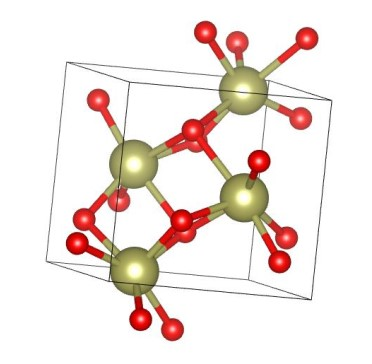
\includegraphics[height=80px]{img/POSCAR.jpg}
        \vspace {12px}
        \caption {Моноклинный \(HfO_2\)}
    \end{figure}

\end{multicols}

\end{frame}

%Слайд с ионными реакциями
\begin{frame}{Ионные реакции}
    \begin{figure}

        \centering
        \includegraphics[height=40px]{schemes/reacts/types.pdf}

    \end{figure}

    \begin {multicols} {2}
    \begin{figure}

        \centering
        \includegraphics[width=100px]{schemes/reacts/R1.pdf}
        \caption{реакция R1}
        
    \end{figure}
    
    \begin{figure}

        \centering
        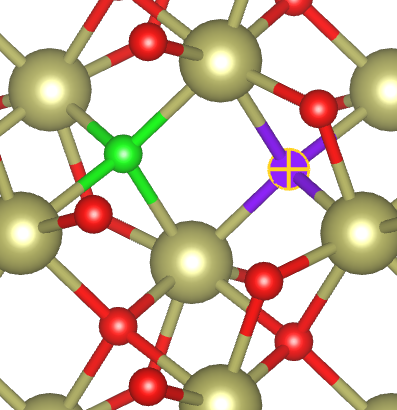
\includegraphics[width=100px]{schemes/reacts/R2.pdf}
        \caption{реакция R2}

    \end{figure}
    \columnbreak
    \begin{figure}

        \centering
        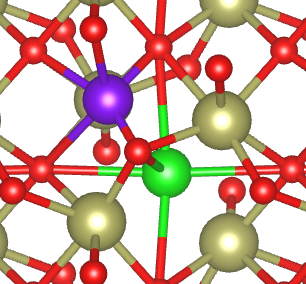
\includegraphics[width=100px]{schemes/reacts/R3.pdf}
        \caption{реакция R3}

    \end{figure}
    \begin{figure}

        \centering
        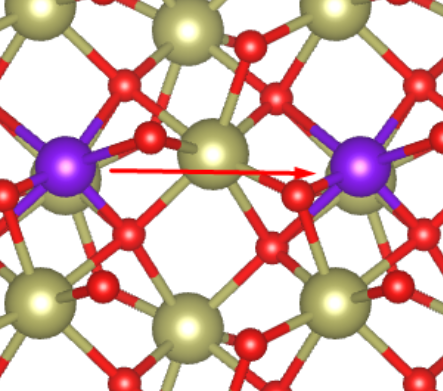
\includegraphics[width=100px]{schemes/reacts/R4.pdf}
        \caption{реакция R4}

    \end{figure}
    \end{multicols}


\end{frame}

% %Слайд для описания электронных реакций
% \begin{frame}{Электронные реакции}



% \end{frame}

%Слайд для формул, описывающих разные ракции

\begin{frame}{Математические основы модели} {Кинетический метод Монте-Карло}

\small

В текущем состоянии системы возможно N реакций.

Выбирается одна реакция, которая произойдет за текущий шаг КМК

Для каждой i-той реакции известна частота: 
\(F_i\)

Частичная сумма частот реакций:
\[S_i = \sum_{j=1}^{i}{F_j}\]

Полная сумма:

\[S = S_N\]

$R$ - случайное число, с равномерным распределением на $[0,S]$

Тогда $j$ - номер реакции, если:
\[S_j \le R < S_{j+1}\]

Время, которое занимает этот шаг:
 \[\frac{1}{S}\]

\end{frame}

% Для ионных реакций:

\begin{frame}{Математические основы модели} {Частоты реакций}

    \small

    Напряжение в любой точке находится как:

    \[U = \frac{l\cdot U_{cond}}{D}+U_{evald}\],

    где \(U_{cond}\) - Напряжение между электродов, \(l\) - расстояние до положительного электрода, \(D\) - расстояние между электродами, а \(U_{evald}\) - периодический потенциал, рассчитанный с помощью метода Эвальда.

    Частоты протекания ионных реакций находятся по формуле:

    \[F = F_0 \cdot \exp{(-\frac{E-\Delta q \Delta a \Delta U}{k_bT})}\],

    где T - температура, \(k_b\) - постоянная больцмана, E - барьер реакции, \(\Delta q\) - переносимый заряд, \(\Delta a\) - расстояние, на которое заряд переносится, \(\Delta U\) - напряжение между начальным и конечным положением, \(F_0\)  - базовая частота реакции.
    

    
\end{frame}


%Используемые в модели константы
\begin{frame}{Константы}
    % \begin{table}
    %     \begin{tabular}{llc}
    %       Константа & Величина\\ 
    %       * & *\\
    %       * & *\\
    %       * & *\\
    %     \end{tabular}
    %     \caption{Базовые константы}
    %   \end{table}

      \begin{table}
        \begin{tabular}{llc}
          Название реакции & Барьер Перехода (эВ) & Базовая частота (Гц)\\ 
          R1 &  \(3.0\) &  \(10^{10}\)\\
          R2 &  \(0.8\) &  \(10^{10}\)\\
          R3 &  \(0.8\) &  \(10^{10}\)\\
          R4 &  \(0.8\) &  \(10^{10}\)\\
          E1 &  \(0.3\) &  \(10^{13}\)\\
          E2 &  \(0.3\) &  \(10^{13}\)\\
          E3 &  \(0.3\) &  \(10^{13}\)\\
        \end{tabular}
        \caption{Константы реакций}
      \end{table}


\end{frame}

% \begin{frame} {Найденные барьеры}

%     \begin {multicols}

%     \begin{figure}

%         \centering
%         \includegraphics[width=100px]{img/barrier/R1}
%         \caption{Барьер R1}

%     \end{figure}

%     \begin{figure}

%         \centering
%         \includegraphics[width=100px]{img/barrier/R1}
%         \caption{Барьер R2}

%     \end{figure}
%     \columndreak

%     \begin{figure}

%         \centering
%         \includegraphics[width=100px]{img/barrier/R1}
%         \caption{Барьер R3}

%     \end{figure}

%     \begin{figure}

%         \centering
%         \includegraphics[width=100px]{img/barrier/R1}
%         \caption{Барьер R4}

%     \end{figure}
%     \end{multicols}
    
% \end{frame}

%Слайд с видом всей смоделированной структуры

% \begin{frame}{Смоделированная структура}
%     \begin{figure}
%         \centering
%         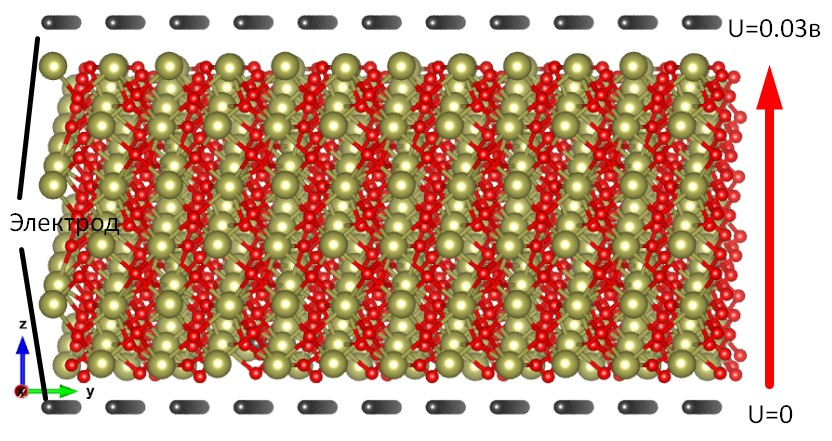
\includegraphics[width=300px]{img/model-result-v3.jpg}
%     \end{figure}

% \end{frame}

%На этом слайде будут/ет картинка с полученным филаментом.
\begin{frame}{Филамент}{после 50000 шагов}

\begin {multicols} {3}
\begin{figure}

    \centering
    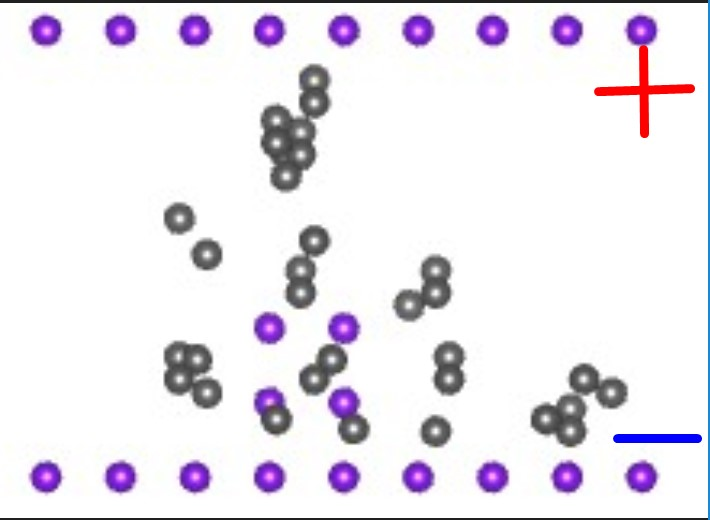
\includegraphics[height=70px]{img/filament/filament__1.jpg}
    \caption{Филамент при напряжении 0.05В между электродами\( ^*\)}
\end{figure}

\columnbreak
\begin{figure}
    \centering
    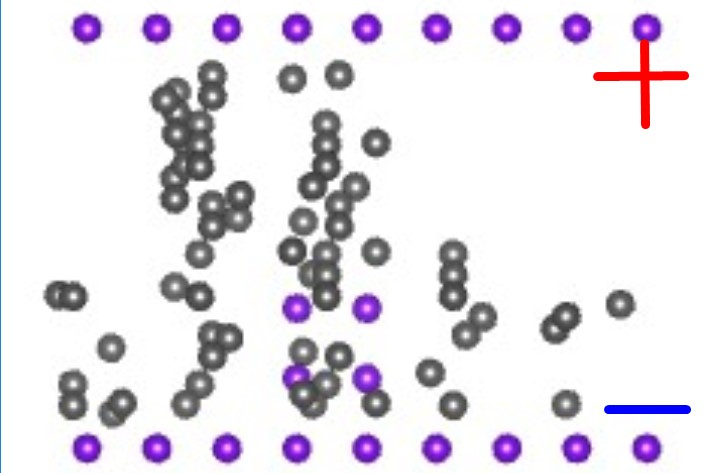
\includegraphics[height=70px]{img/filament/filament__2.jpg}
    \caption{Филамент при напряжении 0.20В между электродами\( ^*\)}
\end{figure}
\columnbreak
\begin{figure}
    \centering
    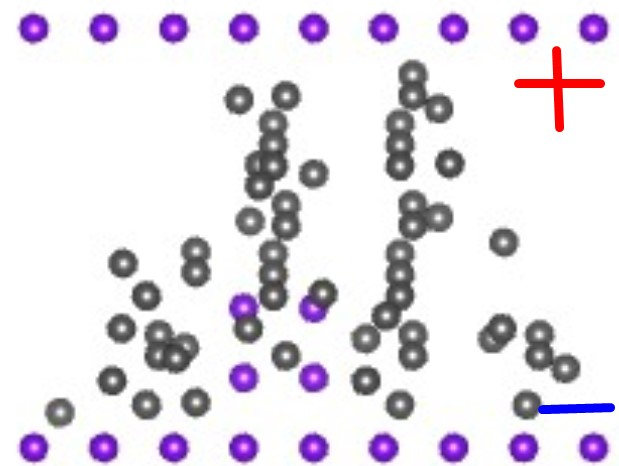
\includegraphics[height=70px]{img/filament/filament__3.jpg}
    \caption{Филамент при напряжении 0.030В между электродами\( ^*\)}
\end{figure}
\end {multicols}
\begin {multicols} {4}
\begin{figure}
    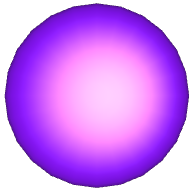
\includegraphics[width=10px]{img/filament/electrode.png}
\end{figure} 
\columnbreak
Электрод
\columnbreak
\begin{figure}
    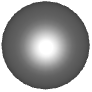
\includegraphics[width=10px]{img/filament/hafnium.png}
\end{figure}

\columnbreak
Вакансия
\end{multicols}
* Толщина среза 12 \r{A}
\end{frame}

%Есть надежда получить реакции set-reset и показать их оттельно, но пока еще нет.
\begin{frame}{ВАХ смоделированной системы}
    Была проведена симуляция системы при разных напряжениях и начальных условиях.
    Это позволило получить Вольт-амперную характеристику.
    \begin {multicols}{2}
        \begin{figure}
            \centering
            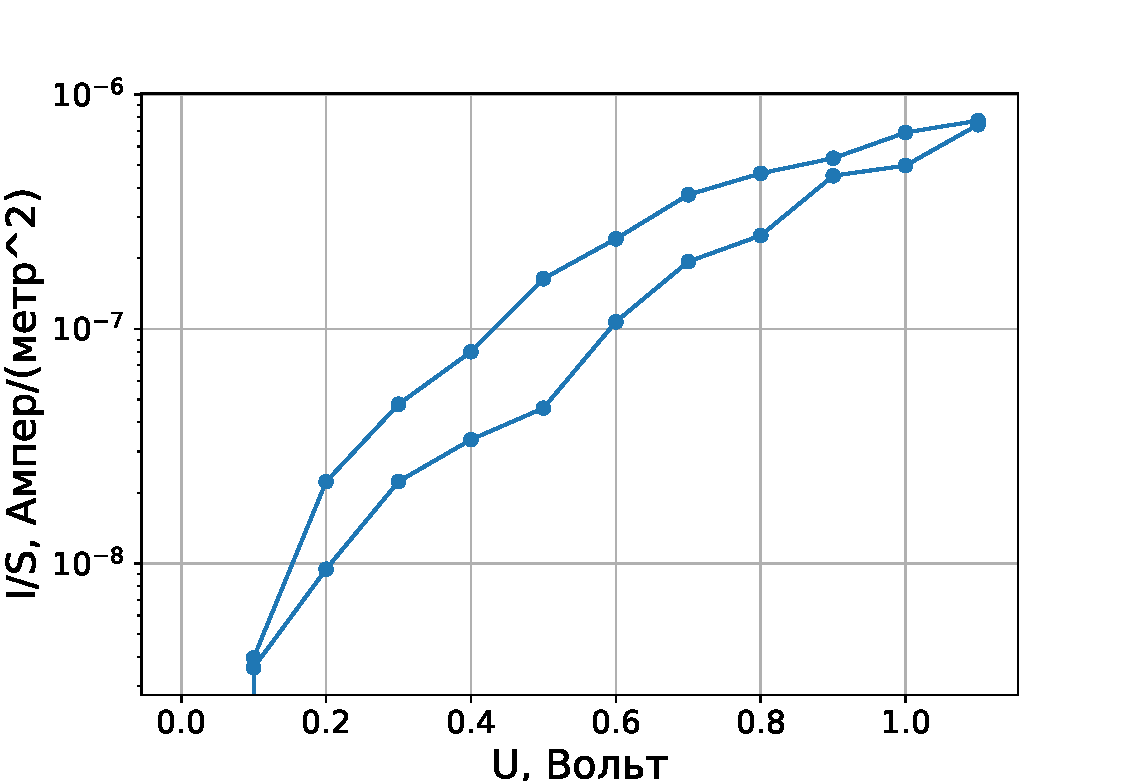
\includegraphics[width=170px]{img/SET.pdf}
            \caption {Процесс SET}
        \end{figure}
        \columnbreak
        \begin{figure}
            \centering
            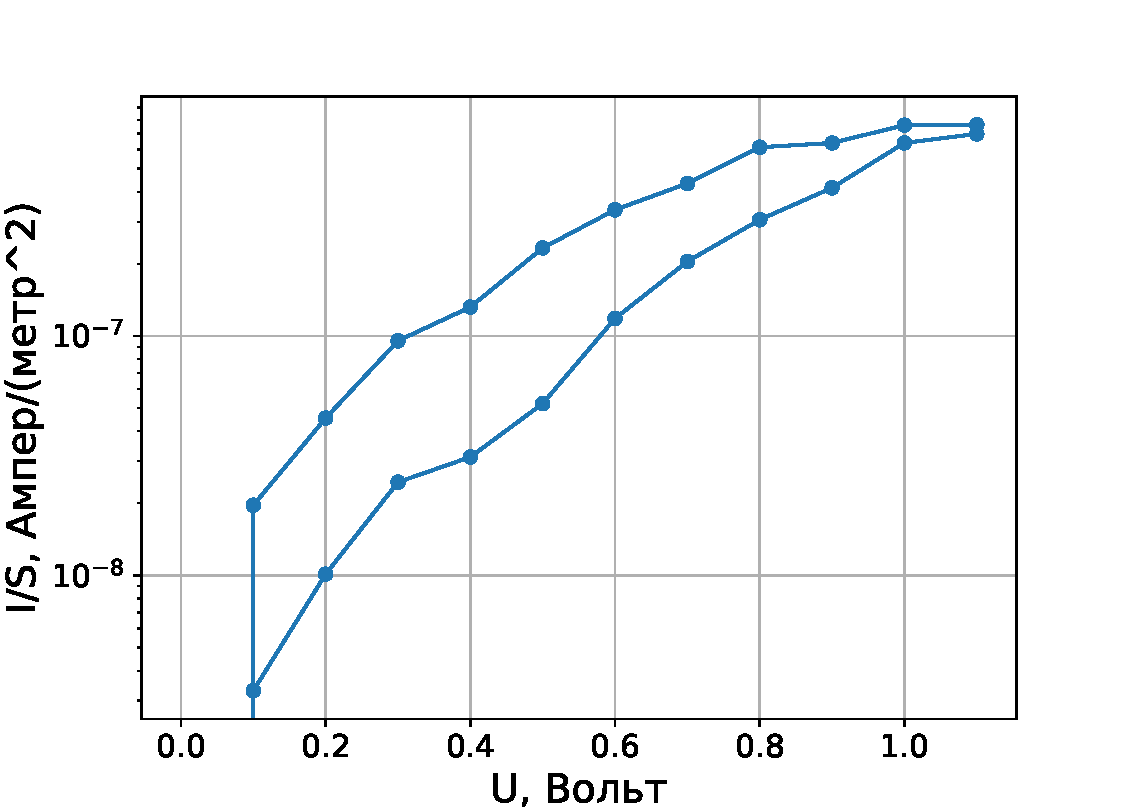
\includegraphics[width=170px]{img/RESET.pdf}
            \caption {Процесс RESET}
        \end{figure}   
    \end{multicols}

\end{frame}

%Слайд с обобщенными результатами
\begin{frame}{Результаты}

\begin{list}{*}{}
    \item  Разработана и реализована модель для симуляции роста филаментарных структур с использованием кинетического метода Монте-Карло
    \item  С использование теории функционала плотности выполнены рассчеты для параметризации процессов.
    \item  Работа модели была проверена, и на её основании было получены и продемонстрировано образование филаментарной структуры при наличии внешнего поля.
\end{list}
\end{frame}
%Слайд с тем, что еще можно сделать
\begin{frame}{Планы}

\begin{list}{*}{}
    \item  Учет сложной структуры интерфейса на границе Оксид-Электрод
    \item  Рассмотрение разных форм электрода.
    \item  Рассмотрение разных веществ в качестве электрода/диэлектрика.
    \item  Изучение вклада от разных способов течения тока в общий ток.
\end{list}



\end{frame}

\begin{frame}[plain]
\vfill
\centerline{Спасибо за внимание!}
\vfill\vfill
\end{frame}

%Секретный слайд
%Секретный - потому, что пока показывать во время основной презентации не планирую
\begin{frame}{Set-Reset в мемристоре}
    \begin{figure}
        \centering
        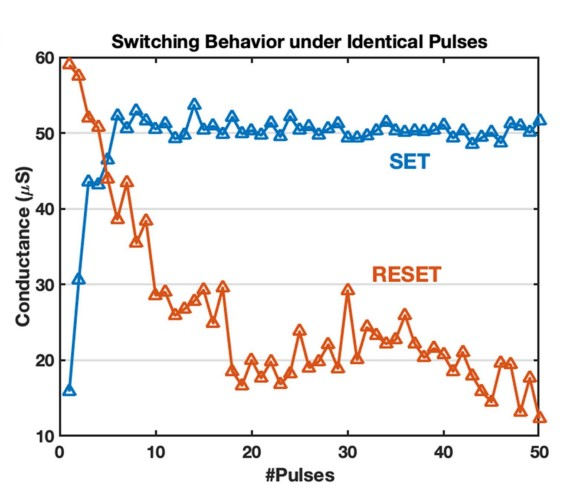
\includegraphics[width=180px]{img/memristor-set-reset.jpg}
        \caption{Set-reset в мемристоре%
    \footnote{%
    Guo Y, Wu H, Gao B and Qian H(2019) Unsupervised Learning on Resistive Memory Array Based Spiking Neural Networks. Front. Neurosci. 13:812. doi: 10.3389/fnins.2019.00812
    }%
  }
    \end{figure}
\end{frame}


\end{document}